\chapter{Case Study at Ikayzo} \label{Chapter:EvaluationInIkayzo}

This chapter outlines a case study of software project telemetry that will be performed at Ikayzo\footnote{http://www.ikayzo.org} with open-source project developers. Open-source project development environment is different from those in classroom or CSDL. The development is collaborated by geographically dispersed developers and project decisions are decentralized. It presents significant challenge for software project telemetry technology to be adopted.

This chapter begins with a description of Ikayzo in Section \ref{EvaluationInIkayzo:Setting}.
Section \ref{EvaluationInIkayzo:Design} outlines the design and strategies of this case study and offers rationale for the decisions.
Section \ref{EvaluationInIkayzo:DataAnalysis} introduces data collection and analysis procedures.
Section \ref{EvaluationInIkayzo:Role} describes researcher's role.
Section \ref{EvaluationInIkayzo:Threats} discusses the limitations and threats. 
The expected results are described in Section \ref{EvaluationInIkayzo:Results}. 
%and the time frame of this case study is given in Section \ref{EvaluationInIkayzo:TimeFrame}.



%%%%%%%%%%%%%%%%%%%%%%%%%%%%%%%%%%%%%%%%%%%%%%%%%%%%%%%%%
%                                                       %
%                   S E C T I O N                       %
%                                                       %
%%%%%%%%%%%%%%%%%%%%%%%%%%%%%%%%%%%%%%%%%%%%%%%%%%%%%%%%%
 
\section{Ikayzo Setting} \label{EvaluationInIkayzo:Setting}

Ikayzo provides open-source projects with free hosting service, which includes source code version control, issue tracking and management, automated metrics collection and analysis, and wiki discussion board. All projects have to go through a screening process before they are hosted. Beyond that, Ikayzo does not participate in or have influence on the decision-making process of the hosted projects.

The metrics collection and analysis support is provided through the software project telemetry system. Unlike the case in the two previous studies where the developers have to install sensors and invoke telemetry analysis themselves, the software project telemetry system is hidden at Ikayzo in order to completely eliminate metrics collection and analysis overhead from the developers. I installed the sensors and pre-configured several telemetry charts. A background daemon process runs the telemetry analyses and updates the charts automatically every night. Users access telemetry metrics analysis results through a link on the web portal for each project. Figure \ref{fig:IkayzoTelemetryReport} shows the exposed telemetry analysis page for one of the projects.

\begin{figure}[p]
  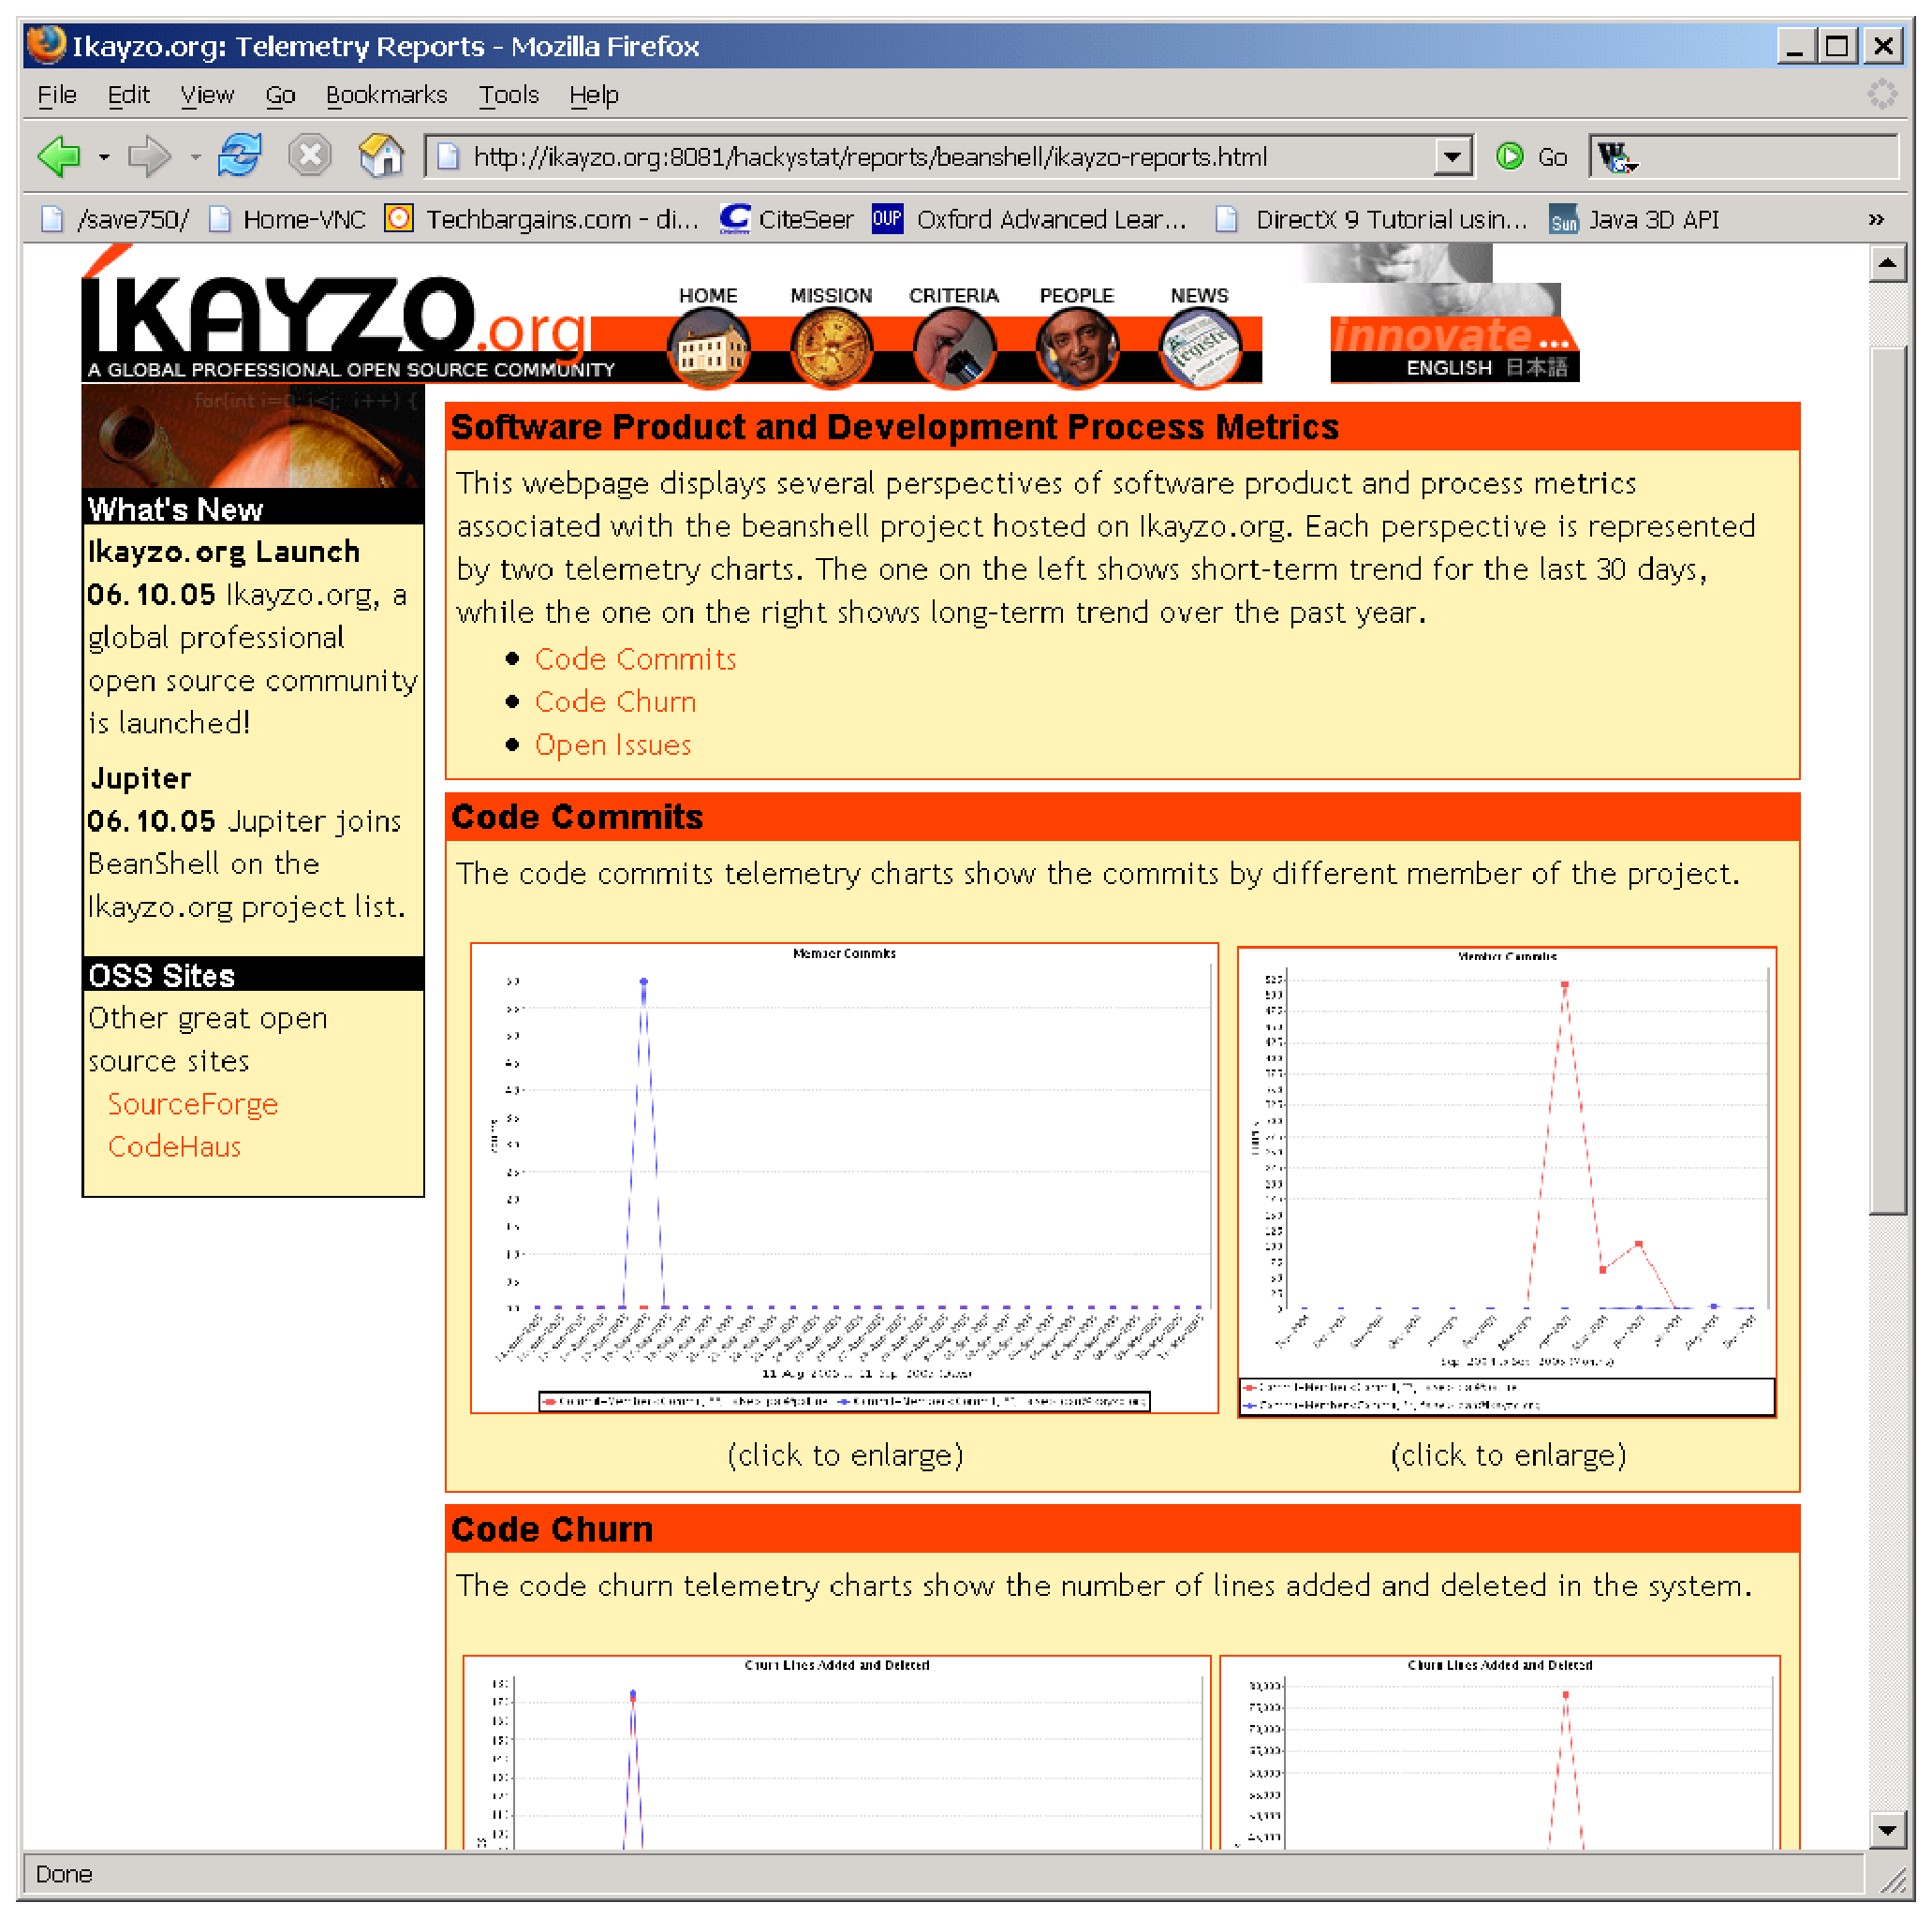
\includegraphics[width=1.00\textwidth]{figures/IkayzoTelemetryReports}
  \caption{Telemetry Reports for Ikayzo Hosted Project} 
  \label{fig:IkayzoTelemetryReport}
\end{figure}

Since the preliminary investigation by Ikayzo and me indicates that most developers are cautious about having their personal software process data being collected, such as which files they are editing at what time, we decided to only install server-side sensors. ``Server-side sensors'' refers to those sensors that monitor activities of various server systems, such as version control server, bug tracking and issue management server. Currently the following metrics are collected: (1) source code commit metrics, and (2) bug and issue metrics. We are planning to add source code size metrics in the near future. These metrics are all public knowledge because everybody can check out source code and browse project issue database through the web. What the software project telemetry system does is essentially make these aspects of the development process more transparent using telemetry charts.


The other services provide by Ikayzo are very much like those provided by other project hosting sites such as \textit{sourceforge.net} or \textit{java.net}, except that Ikayzo is much smaller in scale. As of this writing three projects are hosted by Ikayzo:

\begin{itemize}

	\item \textbf{BeanShell} is a small embeddable interpreter for a Java syntax compatible scripting language for the Java platform. The project has passed JSR-274 voting process, and is heading toward getting included in the Java Standard Edition at some point in the future.

	\item \textbf{Jupiter} is an Eclipse plug-in that provides code review and reporting functionality. It allows management of code annotations stored in XML based files, which can be shared by a development team.
	
	\item \textbf{SDL} stands for simple declarative language. It aims to provide an easy way to describe lists, maps, and trees of typed data in a compact, easy to read representation. Due to its simple API, it is a compelling alternative to XML for property files, configuration files, logs and simple serialization requires.	

\end{itemize}








%%%%%%%%%%%%%%%%%%%%%%%%%%%%%%%%%%%%%%%%%%%%%%%%%%%%%%%%%
%                                                       %
%                   S E C T I O N                       %
%                                                       %
%%%%%%%%%%%%%%%%%%%%%%%%%%%%%%%%%%%%%%%%%%%%%%%%%%%%%%%%%

\section{Case Study Design and Strategies} \label{EvaluationInIkayzo:Design}

Open-source software development environments differ from more traditional centralized software development environment in that development is performed through volunteer work, which makes it impossible to mandate what kind of technology should be used in development process. Both my previous experience and initial investigation at Ikayzo suggest that developers are cautious about their personal process data being collected. As a result, the approach employed at Ikayzo is to avoid those sensitive personal process data. The software project telemetry system is used only to collect and analyze metrics from publicly available source such as project source code repository and issue tracking system, and make these aspects of the development process more transparent by presenting them in a more useful telemetry format.

The goal of this case study is multiple:

\begin{itemize}
	\item To understand the adoption barrier of software project telemetry in an open-source environment where software development is collaborated through geologically-dispersed volunteer work and the decision-making process is decentralized. %All of which makes it infeasible to mandate the technology to be used. The experience with respect with the adoption barrier will not only help me to promote software project telemetry to an open source development environment, but other environment as well.
  \item To observe how software project telemetry is used in open-source development and find out what works and what does not work. 
	\item To understand both technical and social constraints of collection and analysis of different types of metrics in such an environment. 
%	\item To understand the administration cost associated with the current implementation of software project telemetry. 
\end{itemize}

%[Evaluation Strategy]
The evaluation in this case study will adopt the mixed methods paradigm. Since this will be largely a naturalistic study exploring how people use software project telemetry in an open-source development environment, priority will be given to qualitative information obtained during the course of this case study. 

The two most popular approaches in qualitative data collection are survey and ethnographic observation. Though ethnography has the advantage of enabling to observe how developers actually interact with software project telemetry and make project management and process improvement decisions, it is not chosen because of the fact that the open-source developers under this case study contribute to the projects through volunteer effort at their personal time from different locations. As a result, survey method is the only feasible choice to gather feedback. 

The decision to use survey method implies that I have to rely on the developers' self-reported opinions to evaluate software project telemetry. This threat can be mitigated by reconciling survey results with other data. Another source of data is quantitative information from telemetry report request log. If I find evidence that the developers look at telemetry report regularly, then I can put more confidence in their answers when they say software project telemetry is useful or not useful.




%Project metrics are another source of quantitative data, but I doubt they will be interesting since the projects are not that active.

%Software project telemetry system administration effort --- Since I am the person responsible for providing automated metrics collection and analysis support to projects hosted by Ikayzo, I am keeping a detailed diary of the effort I spend performing my task. I am the developer of software project telemetry reference implementation and various components in Hackystat framework, I am quite familiar with the system. My effort can be viewed as the lower bound of providing software project telemetry metrics support to an organization. I will reflect the difficulties I encountered, which are the potential adoption barriers of the technology.




%%%%%%%%%%%%%%%%%%%%%%%%%%%%%%%%%%%%%%%%%%%%%%%%%%%%%%%%%
%                                                       %
%                   S E C T I O N                       %
%                                                       %
%%%%%%%%%%%%%%%%%%%%%%%%%%%%%%%%%%%%%%%%%%%%%%%%%%%%%%%%%

\section{Data Collection and Analysis Procedures} \label{EvaluationInIkayzo:DataAnalysis}

This case study will collect data from two sources:
\begin{itemize}
	\item Qualitative data from surveys of the developer's opinion about software project telemetry. 
	\item Quantitative information about telemetry report requests.
\end{itemize}

The two sources of data will be integrated at data interpretation phase with emphasis on qualitative information and quantitative data corroborating the qualitative findings.





\subsection{Surveys}

Different approaches can be used to conduct a survey such as questionnaire or interview. In this case study, email questionnaires will be used for BeanShell project, and interviews will be used for Jupiter and SDL project. The reason is that the BeanShell project members are on the mainland and I don't have a chance to meet them in person, while I am able to meet other project members on a regular basis.

The survey, regardless of the approach chosen, will be conducted on a monthly basis. The purpose is to find out the developer's opinion about software project telemetry. The survey will follow the following basic steps:

\begin{itemize}
  \item Ask the developers how often they view telemetry reports. 
	\item Review telemetry reports together with the developers (omitted in email questionnaire).
	\item Find out what they think when they see the telemetry reports, and ask them whether the reports reflects the overall direction of the projects or not.
	\item Ask them what other telemetry analysis might be useful to them.
	\item Gradually introduce other available sensors and find out whether people are interested and under what condition they will use those sensors.
	\item Gradually reveal the regular telemetry analysis interface hidden underneath Ikayzo project portal which allow people to experiment with metrics themselves, and find out whether they exhibit interest beyond the predefined telemetry reports.
\end{itemize}





  
  

\subsection{Telemetry Report Requests}

Telemetry reports are integrated into the web portal for each project at Ikayzo. There are links on the main web page leading to telemetry charts. I will turn on web server logging facilities to log all telemetry chart requests. The information logged will include requester IP address, request time, and the telemetry chart being requested. The log will tell me the frequency of different telemetry charts being requested.

%This information can be correlated with project product metrics. We might find interesting correlations such as whether projects with constant development invoke telemetry analysis more often.;  (2) The popularity of different telemetry analysis.




%%%%%%%%%%%%%%%%%%%%%%%%%%%%%%%%%%%%%%%%%%%%%%%%%%%%%%%%%
%                                                       %
%                   S E C T I O N                       %
%                                                       %
%%%%%%%%%%%%%%%%%%%%%%%%%%%%%%%%%%%%%%%%%%%%%%%%%%%%%%%%%

\section{Researcher's Role} \label{EvaluationInIkayzo:Role}

Ikayzo uses software project telemetry system to provide automated metrics collection and analysis service to the projects hosted on its site. The system is designed and developed by me as part of my dissertation research. It is distributed under GPL license and everyone can use it free of charge. 

I provide volunteer technical support for Ikayzo running and administering its installation of software project telemetry system. My responsibility includes:
\begin{itemize}
	\item Setting up server-side telemetry sensors for automated metrics collection.
	\item Configuring software project telemetry system.
	\item Defining telemetry reports to present metrics analysis results.
	\item Writing scripts to update and publish telemetry reports automatically. 
	\item Monitoring the sensors and the system to make sure everything is working correctly.
\end{itemize}

My involvement in Ikayzo is strictly confined to providing software project telemetry system technical support. I don't provide support for other Ikayzo services, such as version control, bug tracking, and wiki discussion board. I don't participate in Ikayzo internal administrator. Finally, neither Ikayzo nor I have influence on the decision-making process of the hosted projects. 







%%%%%%%%%%%%%%%%%%%%%%%%%%%%%%%%%%%%%%%%%%%%%%%%%%%%%%%%%
%                                                       %
%                   S E C T I O N                       %
%                                                       %
%%%%%%%%%%%%%%%%%%%%%%%%%%%%%%%%%%%%%%%%%%%%%%%%%%%%%%%%%

\section{Threats, Verification, and Validation} \label{EvaluationInIkayzo:Threats}

\subsection{Measurement Validity}

Possible threat to measurement validity might come from qualitative data with respect to the developer's opinion of software project telemetry, but the risk is low. The reasons are as follows:

\begin{itemize}
	\item Neither Ikayzo nor I can influence the decision-making process and the overall direction of the hosted projects. The developers make volunteer contribution to project development. They don't get paid. There is no incentive for them to misrepresent their true opinions toward software project telemetry.
	
	\item Three open-source projects are involved in this case study. The developers' opinion from different projects will be compared and contrasted.
	
	\item All telemetry report requests are logged. The quantitative information will be used to corroborate the qualitative findings. 
\end{itemize}


\subsection{Internal Validity}

Internal validity refers to causality. In this case study, it is related to whether the telemetry reports have made the developers more aware of the status of the projects and thus contribute to better decision-making. Though this case study relies on the developers' subject opinion about the utility of software project telemetry, the threat is mitigated through the use of multiple data sources: data from 3 different projects, and quantitative and qualitative information from the the same project. All information will be reconciled and cross-validated at data analysis stage.


\subsection{External Validity}

External validity concerns the extent to which the experience gathered from the 3 projects hosted at Ikayzo can be generalized to other open-source development environment. 
The threat is quite low in this case study since the services provided by Ikayzo are pretty standard compared to other open-source project hosts such as \textit{sourceforge.net} or \textit{java.net}. 





%%%%%%%%%%%%%%%%%%%%%%%%%%%%%%%%%%%%%%%%%%%%%%%%%%%%%%%%%
%                                                       %
%                   S E C T I O N                       %
%                                                       %
%%%%%%%%%%%%%%%%%%%%%%%%%%%%%%%%%%%%%%%%%%%%%%%%%%%%%%%%%

\section{Expected Results} \label{EvaluationInIkayzo:Results}

Not all metrics can be collected in an open-source development environment. Some might be feasible to collect technically, but infeasible socially. The case study will allow me to better understand the constraints associated with metrics collection and analysis. The experience gathered in this case study will enhance my understanding of software project telemetry technology adoption barriers, not only in open-source development environments, but also in more closed traditional software development environments.





%%%%%%%%%%%%%%%%%%%%%%%%%%%%%%%%%%%%%%%%%%%%%%%%%%%%%%%%%
%                                                       %
%                   S E C T I O N                       %
%                                                       %
%%%%%%%%%%%%%%%%%%%%%%%%%%%%%%%%%%%%%%%%%%%%%%%%%%%%%%%%%

%\section{Time Frame} \label{EvaluationInIkayzo:TimeFrame}
%
%I expect to start the case study in October 2005. The study will last around four months.
%
%


% -what they want to see
% -what they think when they see the analysis
% -what they do after seeing the analysis.